\subthesischapter{Aspectos conceptuales en la Rehabilitación Muscular}

\subsubthesischapter{Accidentes Cerebrovasculares}
Se define como accidente cerebrovascular (ACV) o Ictus a todo episodio de instauración súbita, aguda o subaguda, en el que, a causa de una lesión primaria o secundaria localizable en cualquier punto del sistema cardiovascular, se produce un déficit neurológico, permanente o transitorio, en relación con la zona afectada~\cite{ictus}.

\subsubthesischapter{Tipos de afecciones motoras y cognitiva}
Los tipos y grados de discapacidad que siguen a un derrame dependen de qué área del cerebro esté dañada (ver Figura~\ref{fig: cerebralcortex}). Generalmente, el accidente cerebrovascular puede causar cinco tipos de discapacidades: parálisis o problemas para controlar el movimiento; trastornos sensoriales, incluyendo dolor; problemas en el uso o comprensión del lenguaje; problemas con el pensamiento y la memoria, y trastornos emocionales~\cite{post-strok}. 

\begin{figure}[ht]
    \centering
    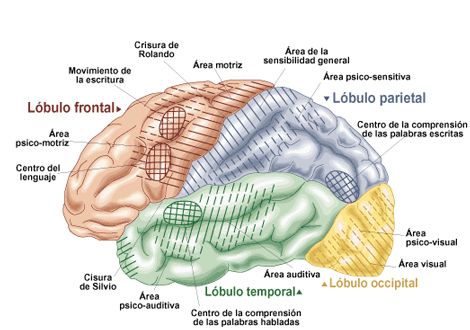
\includegraphics[scale=0.5]{images/brain.jpg}
    \caption{Áreas funcionales de la corteza cerebral.}
    (Tomado de ~\cite{areacereabral})
    \label{fig: cerebralcortex}
\end{figure}

\begin{itemize}
    \item Parálisis o problemas para controlar el movimiento:
    
    La parálisis es una de las discapacidades más comunes causadas por un accidente cerebrovascular. Se suele dar en el lado del cuerpo opuesto al lado del hemisferio   dañado y puede afectar a la cara, un brazo, una pierna o a todo un lado del cuerpo. Esta parálisis unilateral se denomina hemiplejia (si la parálisis no es completa se denomina hemiparesia). Los pacientes con hemiparesia o hemiplejia pueden tener dificultades con las actividades cotidianas, como caminar o agarrar objetos~\cite{cuidadosalpacienteadulto}.

    \item Alteraciones sensoriales, incluyendo dolor:
    
    Los pacientes con accidente cerebrovascular pueden perder la capacidad de sentir el tacto, dolor, temperatura o posición. También pueden tener dificultad para reconocer objetos que están sosteniendo, e incluso pueden ser lo suficientemente graves como para causar la pérdida del reconocimiento de su propia extremidad. Algunos pacientes con apoplejía llegan a experimentar dolor, entumecimiento o sensaciones extrañas de hormigueo o picor en las extremidades paralizadas o debilitadas, un síntoma conocido
    como parestesias~\cite{post-strok}.
    
    \item Problemas para usar o comprender el lenguaje (afasia):
    
    Los sobrevivientes de accidentes cerebrovasculares experimentan deficiencias en el lenguaje, que involucran la capacidad de hablar, escribir y comprender el lenguaje hablado y escrito. En las personas diestras, estos accidentes cerebrovasculares generalmente involucran el lado izquierdo del cerebro. Una lesión inducida por un accidente cerebrovascular en cualquiera de 
    los centros de control del lenguaje del cerebro puede afectar gravemente la comunicación verbal. Según~\cite{post-strok} existen varios tipos de afasia:
    \begin{itemize}
        \item Afasia expresiva, en la que las personas pierden la capacidad de hablar o escribir las palabras que están pensando y de juntar palabras en oraciones coherentes y gramaticalmente correctas.
        \item Afasia receptiva, en la que las personas tienen dificultad para comprender el lenguaje hablado o escrito y, a menudo, tienen un habla incoherente. Aunque estos individuos pueden formar oraciones gramaticalmente correctas, sus expresiones a menudo carecen de significado.
        \item Afasia global, en la que las personas pierden casi todas sus habilidades lingüísticas; no pueden entender el lenguaje o usarlo para transmitir pensamientos.  
    \end{itemize}

    \item Problemas con el pensamiento y la memoria:
    
    Un accidente cerebrovascular puede causar daño a partes del cerebro responsables de la memoria, el aprendizaje y la conciencia. Los pacientes pueden haber reducido dramáticamente su capacidad de atención o pueden experimentar déficit en la memoria a
    corto plazo. También pueden perder su capacidad de hacer planes, comprender el significado de las cosas, aprender nuevas tareas, o participar en otras actividades mentales complejas~\cite{post-strok}.
    
    \item Trastornos emocionales:
    
    Muchas personas tras sobrevivir a un derrame sienten miedo, ansiedad, frustración, ira, tristeza y un sentimiento de dolor por sus pérdidas físicas y mentales. Estos sentimientos son una respuesta natural al trauma psicológico del ictus. Algunos trastornos emocionales y cambios de personalidad son causados por los efectos físicos del daño cerebral~\cite{post-strok}. 
\end{itemize}

\subsubthesischapter{Activación muscular durante el pedaleo}
Muchos estudios de ciclismo han utilizado las señales de electromiografía (EMG) para comprender mejor cómo funcionan los músculos durante las diferentes fases del movimiento. Una de las particularidades observadas ocurre durante la fase de propulsión del pedaleo, donde la
mayoría de los pares de músculos agonistas/antagonistas se activan juntos para generar torques durante esta fase. El análisis está basado en los tiempos de inicio y final de la contracción muscular y los niveles de amplitud alcanzados, sincronizados con mediciones cinemáticas o dinámicas del movimiento como el ángulo, la aceleración o la velocidad angular, torque, potencia o de marcadores de tiempo con el uso de codificadores en la manivela de la bicicleta o del pedal motorizado. Con ellos se ha demostrado que las
personas sanas tienen patrones de coordinación intermusculares predecibles durante el pedaleo; los cuales también están relacionados con la cadencia o revoluciones por minutos, la posición del cuerpo, así como con la carga de entrenamiento a la cual es sometido el usuario. Estos patrones suelen ser alterados en pacientes con discapacidades motoras debido a cambios que sufren los músculos, por ejemplo el acortamiento ~\cite{johnston2007biomechanical}. De ahí que la señales de EMG permiten detectar los grupos musculares dañados y enfocar el entrenamiento hacia estos ~\cite{hug2009electromyographic, kautz1998relationships}


Según~\cite{Losmúscu21}, los grupos musculares que intervienen en el pedaleo son:
\begin{itemize}
    \item \textbf{Los cuádriceps} son un grupo de cuatro músculos situados en la parte frontal del muslo. Estos músculos incluyen el recto femoral (RF), el vasto lateral (VL), el vasto intermedio (VI) y el vasto medial (VM). Durante el pedaleo, los cuádriceps se contraen para extender la pierna en la rodilla durante la fase de empuje hacia abajo del pedal. Esta acción proporciona la potencia necesaria para superar la resistencia y avanzar con eficiencia.
    
    \item Situados en la parte posterior del muslo, \textbf{los isquiotibiales} son otro grupo muscular clave en el pedaleo. El bíceps femoral (BF), el semitendinoso (ST) y el semimembranoso (SM) son los músculos principales de esta zona. Durante la fase de levantamiento del pedal, los isquiotibiales se activan para flexionar la pierna en la rodilla y extender la cadera. Este movimiento se encarga de levantar el pedal y preparar la siguiente fase de empuje.
    
    \item \textbf{Los gemelos} (GM, GL) y \textbf{el sóleo} (SOL) se encuentran en la pantorrilla y también participan en el pedaleo. Son cruciales para la flexión plantar del pie durante la fase de empuje hacia abajo del pedal. Su acción ayuda a generar potencia y proporciona estabilidad en el tobillo durante el pedaleo.
    
    \item Localizados en la parte frontal de la espinilla, \textbf{los tibilales anteriores} (TA) intervienen en la flexión dorsal del pie durante la fase de levantamiento del pedal. Esta acción es esencial para mantener el equilibrio y preparar la pierna para el siguiente empuje.
    
    \item Aunque su papel es menos evidente, los \textbf{glúteos} (G) también son importantes en el pedaleo. Tanto el glúteo mayor como el glúteo medio contribuyen a la extensión de la cadera y ayudan a potenciar el movimiento durante la fase de empuje del pedal.
\end{itemize}

La Figura~\ref{fig: musculegroups} muestra detalles gráficos de los grupos musculares mencionados.

\begin{figure}[ht]
    \centering
    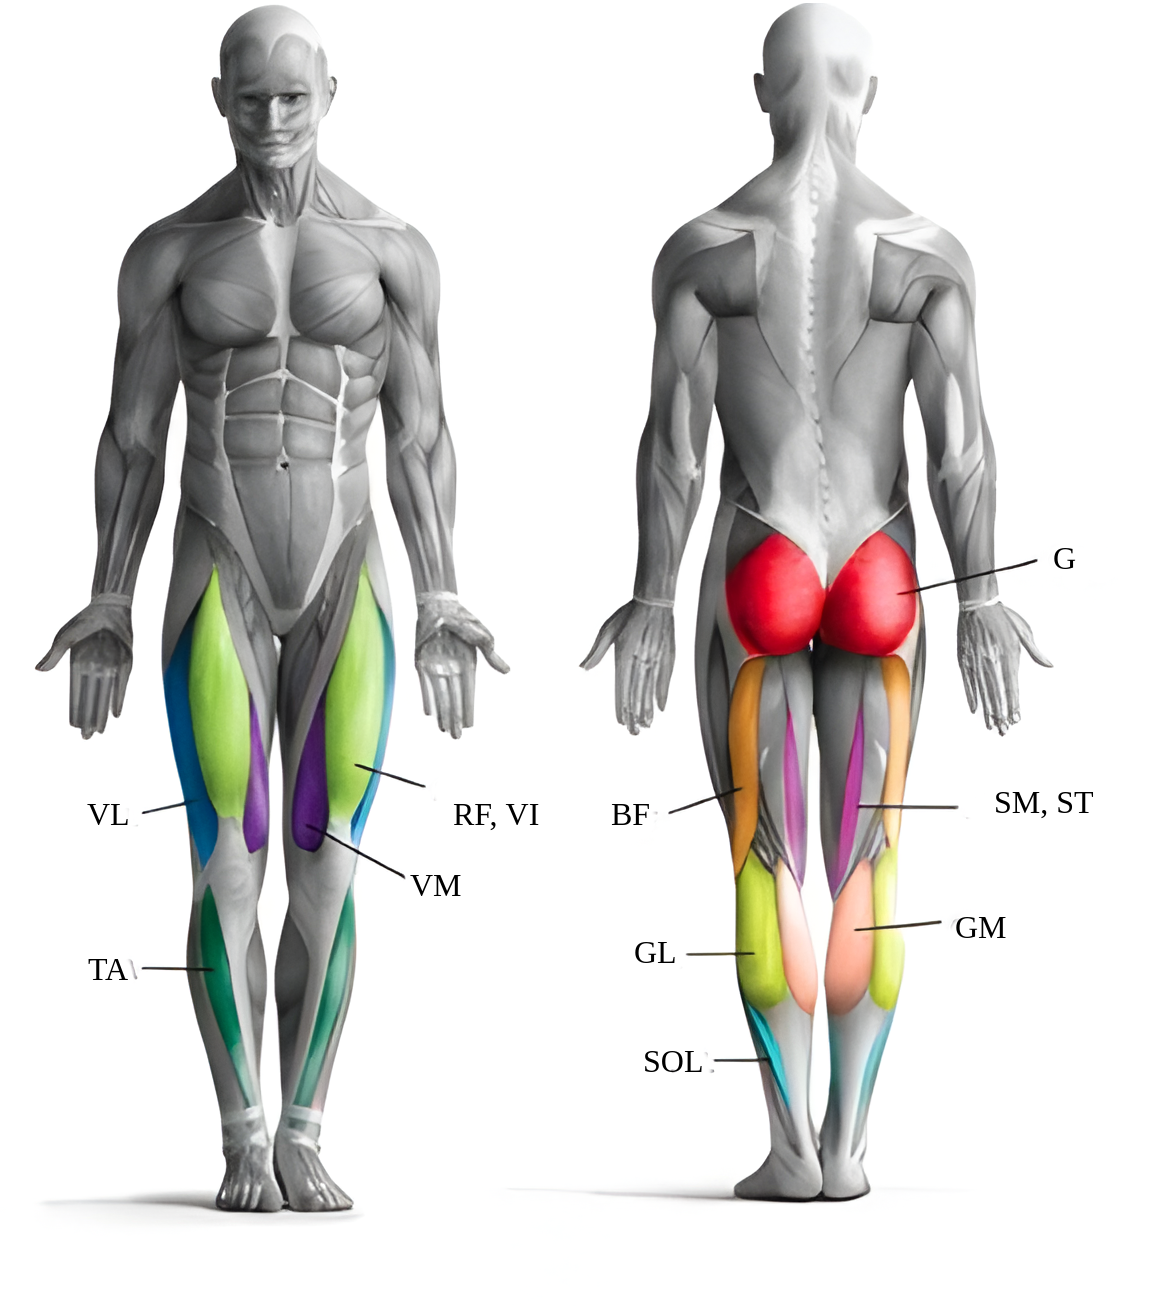
\includegraphics[scale=0.17]{images/musculegroups.png}
    \caption{Grupos musculares usados en pedaleo.}
    (Tomado de ~\cite{Quémúsc72})
    \label{fig: musculegroups}
\end{figure}

\subsubthesischapter{Tecnologías de la Rehabilitación}
Las denominadas tecnologías en rehabilitación se pueden concebir como el conjunto de productos y conocimientos desarrollados desde avances tanto en la ingeniería de la rehabilitación como en las profesiones y disciplinas que estudian el fenómeno de la discapacidad. En este orden de ideas, la tecnología en rehabilitación estudia no sólo lo relacionado con el desarrollo y la producción de instrumentos, equipos, sistemas o dispositivos que contribuyan a procesos de rehabilitación, sino que se interesa, además, por el impacto de estos elementos en el desempeño y la capacidad funcional de las personas con discapacidad, en el acceso de estas personas y sus familias a los adelantos tecnológicos y el nivel de uso que se les da, además de lo relacionado con la accesibilidad y diseño~\cite{matheus1990tecnologia}.

Un término que regularmente se utiliza en este campo es la tecnología de asistencia, que no debe igualarse al de ingeniería de la rehabilitación ni al de tecnología de la rehabilitación, órtesis o prótesis, pues no son idénticos. En esta perspectiva Bronzino y cols.~\cite{enderle2012introduction} mencionan que:

\begin{itemize}
    \item  La tecnología de asistencia es la utilización de cualquier parte de un equipo o sistema productivo modificado o comercializado, para incrementar o mejorar capacidades funcionales de un individuo. Esta definición ve la tecnología de asistencia como una serie de aparatos, estrategias y/o servicios, que ayudan al individuo a realizar mejor una actividad; en consecuencia, incluye desde baja tecnología, que es poco costosa, hasta alta tecnología, que es costosa y con productos de compleja fabricación. Como ejemplos de baja tecnología se incluyen utensilios de doble agarre, cepillos para la boca, entre otros; y de alta tecnología aparatos de comunicación computarizada, máquinas lectoras con inteligencia artificial y brazos artificiales.
\end{itemize}

\textbf{Modalidades de Rehabilitación} \\ 
La terapia con dispositivos robóticos de pedaleo se clasifica, al igual que las terapias convencionales, en modo pasivo, activo y activo asistido~\cite{barclay2019effect}. Estos diferentes enfoques se prescriben según el grado de las secuelas que padece el paciente, el nivel de conciencia de este y las diferentes fases del proceso de rehabilitación en que se encuentran. El ciclismo con estos fines consiste en que los usuarios ejecuten movimientos circulares, similares a los realizados en una bicicleta.

En el ciclismo activo, la persona al pisar o agarrar el pedal es capaz de continuar el ejercicio por sí solo. Durante esta modalidad, el paciente debe ir venciendo gradualmente las resistencias opuestas al movimiento. De esta manera el tratamiento es denominado como resistido y su objetivo principal es el fortalecimiento de los músculos involucrados. En el modo pasivo, los miembros afectados siguen la trayectoria y velocidad programada para los pedales \cite{ferreira2020virtual}. Este modo es también empleado en la rehabilitación activa asistida, la cual es aplicada a los pacientes que debido a la disminución de la fuerza muscular, inician el movimiento activo pero no son capaces de recorrer todo el arco articular \cite{cruz2009guia}. En este caso las tecnologías de pedaleo permiten la transición de forma automática o manual del entrenamiento activo al pasivo y viceversa.

El ciclismo pasivo es adecuado al principio de la rehabilitación, pues contribuye a la regulación del tono muscular, relajación de la musculatura y prevención de las dificultades que trae consigo estar inactivo o inmovilizado, disminuyendo así las probabilidades de
complicaciones a largo plazo \cite{cruz2009guia}. El inicio temprano de intervenciones de ejercicios de pedaleo desde la cama en pacientes críticamente enfermos puede ayudar a reducir la sarcopenia y recuperar la fuerza muscular \cite{nickels2020acceptability}. También es indicado para reducir la inflamación, aliviar el dolor y recuperar el rango de movimiento. Además, se ha comprobado un mejoramiento en el sistema cardiovascular y respiratorio después de la terapia pasiva \cite{cruz2009guia, phadke2019impact}.
Esta modalidad es particularmente útil en pacientes con déficit severo que no tienen control o potencia motriz suficiente para participar en movimientos activos, por ejemplo, sujetos con lesión medular (LM) completa \cite{phadke2019impact, nardone2017passive}. Phadke y cols \cite{phadke2019impact} reflejaron en una revisión sistemática notables efectos del ciclismo pasivo en miembros inferiores para personas con esta condición. En las intervenciones clínicas analizadas por estos autores, los efectos positivos fueron más evidentes tras la realización de múltiples sesiones. Entre los efectos cardiovasculares, se observó un incremento del flujo sanguíneo en las piernas con la consecuente disminución de la resistencia vascular periférica. En el sistema músculoesquelético, hubo un mantenimiento e incremento del RDM de las articulaciones y una atenuación de la atrofia muscular. Además, fue comprobada la influencia de los ejercicios pasivos en el SNC, donde los indicadores mostraron una disminución significativa de la espasticidad (evaluada tras la medición de la amplitud del reflejo H) y de la inhibición intracortical. En los pacientes con EM, el ciclismo pasivo también ha producido estos efectos antiespásticos \cite{motl2006effect, guyot2012effects}. Todas estas repercusiones generalmente son apreciadas a partir de la realización de pedaleo activo \cite{nardone2016effects}, sobre todo en sujetos sanos, de ahí la importancia de conocer que el pedaleo pasivo también produzca efectos similares.

El ciclismo activo-asistido ha producido mejoras en la función motora de los pacientes con EP, particularmente el temblor y la bradicinesia \cite{ryan2020interval, palomino2021efectividad}. Esta modalidad es aprovechada para su uso con terapias complementarias como la estimulación eléctrica funcional (EEF). Esta técnica ha sido considerada desde hace varios años como un método bien establecido y estandarizada en la rehabilitación de pacientes con enfermedades neurológicas como los ACV \cite{rabelo2018overview}. El ciclismo asistido por EEF es un enfoque utilizado con fines de re-habilitación que contribuye a restaurar el trofismo muscular y aumentar la fuerza muscular \cite{barbosa2015application, ferrante2008cycling}. El principio de funcionamento se basa en estimular las unidades motoras para activar los músculos paralizados o paréticos durante la realización de tareas funcionales. Diferentes estudios han evaluado la eficacia de la EEF combinada con el ciclismo en la recuperación motora, principalmente en pacientes con ACV \cite{ambrosini2020does}, LM \cite{casabona2020effects} y esclerosis múltiple (EM) \cite{pilutti2019functional}. También se ha evidenciado beneficios positivos sobre la capacidad aeróbica máxima, el control postural, la espasticidad y la coordinación motora \cite{barbosa2015application, rabelo2018overview}.